\section{}
\textit{The system shown is assumed to have a rotating imbalance and is operated at 100 rpm and 200 rpm. At 100 rpm the steady state amplitude of vibration is 1 mm while at 200 rpm it is 5 mm.}

\begin{figure}[H]
    \centering
    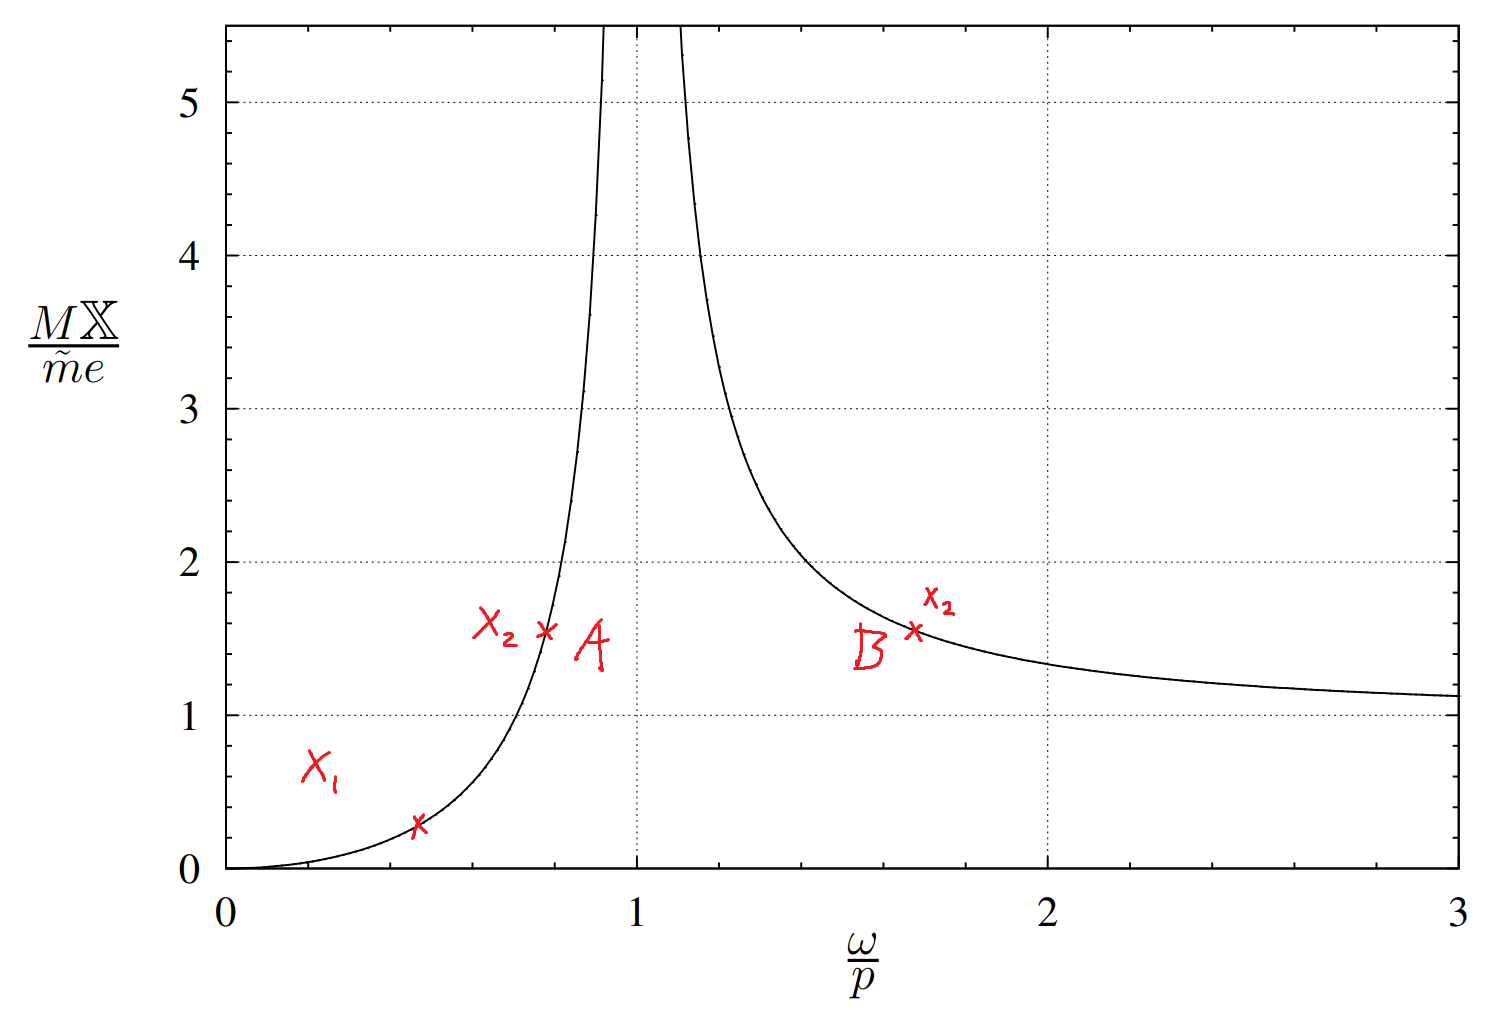
\includegraphics[width=0.5\textwidth]{Questions/Figures/Q3 Frequency Response.png}
    \caption{Frequency response of the system.}
    \label{fig:Q3}
\end{figure}

The system can be operating at either A or B for $\mathbb{X}_2 = 5$ mm. Assuming that the system is operating at A, the system is below resonance, which leads
\begin{align*}
    \frac{M \mathbb{X}_2}{\tilde{m}e} &= \frac{\left(\frac{\omega_2}{p}\right)^2}{1 - \left(\frac{\omega_2}{p}\right)^2} 
\end{align*}
The system at $\mathbb{X}_1 = 1$ mm is operating below resonance, so,
\begin{align*}
    \frac{M \mathbb{X}_1}{\tilde{m}e} &= \frac{\left(\frac{\omega_1}{p}\right)^2}{1 - \left(\frac{\omega_1}{p}\right)^2}
\end{align*}
Solving for $p$,
\begin{align*}
    p_{A} &= 400 \text{ RPM}
\end{align*}

If the system is operating at B, the system is above resonance, which leads
\begin{align*}
    \frac{M \mathbb{X}_2}{\tilde{m}e} &= \frac{1}{\left(\frac{\omega_2}{p}\right)^2 - 1}
\end{align*}
Solving for $p$,
\begin{align*}
    p_{B} &= 163 \text{ RPM}
\end{align*}

\subsection{}
% (5 pts) It is decided to operate the system shown at 200 rpm, however, the amplitude of 
% vibration is too large, and a vibration absorber is to be added.
% ssuming that the natural frequency of the original system is at 150 rpm, what should the 
% mass m2 be as a fraction of m1 to ensure that the lowest natural frequency of the combined 
% system is 100 rpm? 
\textit{It is decided to operate the system shown at 200 rpm, however, the amplitude of vibration is too large, and a vibration absorber is to be added. Assuming that the natural frequency of the original system is at 150 rpm, what should the mass $m_2$ be as a fraction of $m_1$ to ensure that the lowest natural frequency of the combined system is 100 rpm?}

Let the natural frequency of the mass added be $p_{22} = 200$, the frequency of the original system be $p_{11} = 150$, and the frequency of the combined system be $p_{1} = 100$. Then this relation must be satisfied,
\begin{align*}
    \left(\frac{p_{22}}{p_{11}}\right)\left(\frac{p}{p_{22}}\right)^4 - [1 + (1 + \mu) \left(\frac{p_{22}}{p_{11}}\right)^2] \left(\frac{p}{p_{22}}\right)^2 + 1 &= 0 \\
    \left(\frac{200}{150}\right)\left(\frac{100}{200}\right)^4 - [1 + (1 + \mu) \left(\frac{200}{150}\right)^2] \left(\frac{100}{200}\right)^2 + 1 &= 0 \\
\end{align*}
Solving for $\mu$,
\begin{align*}
    \mu &= 0.9375
\end{align*}

